%%%%%%%%%%%%%%%%%%%%%%%%%%%%%%%%%%%%%%%%%%%%%%%%%%%%%%%%%%%%%%%%%%%%%%%%%%%%%%%%
\chapter{Proof of Concepts and Validation}\label{ch:validation}
%%%%%%%%%%%%%%%%%%%%%%%%%%%%%%%%%%%%%%%%%%%%%%%%%%%%%%%%%%%%%%%%%%%%%%%%%%%%%%%%

\section{Emulated Testbeds}


As proof of concepts for our tool, we are going to use Mininet's emulated testbeds. These tests are easily implemented and reproduced, and are able to test the performance on traffic generation realism. Tests in a physical testbeds of, and network functions stays for future work.

This first testbed is a tree topology, and represents tests performed by Swing\cite{swing-paper} found on the literature \cite{background-traffic-matter}\cite{legotg-paper}. The second is much simples, and is just a one hop connection of two hosts. Both topologies are SDN neworks, and have OpenDayLight Beryllium as controller. 


All the traffic is generated by the host \textit{h1} with IPv4 address 10.0.0.1. The traffic will to be captured form the host interface with TCPdump in a pcap format, and just the outgoing traffic will be considered. Any response packet form the hosts will be ignorated, since we want to evaluate just the traffic generated by the host, as it were a replay engine, such as TCPreplay or TCPivo\cite{tcpivo-paper}


\begin{figure}[!ht]
	\centering
	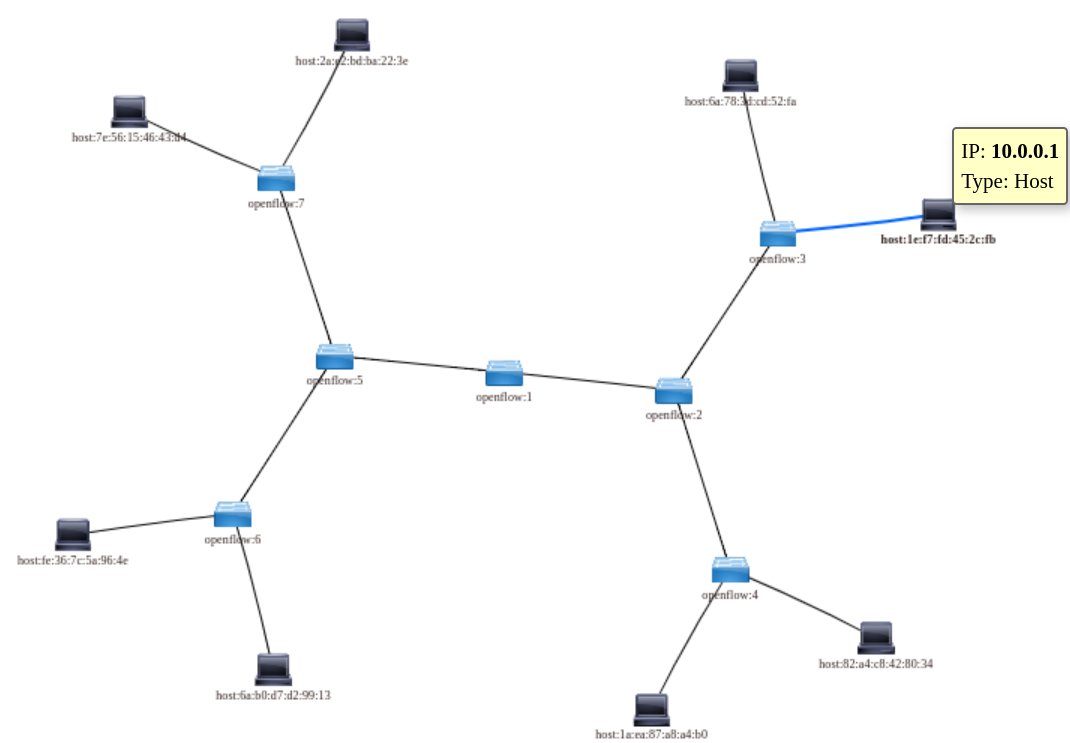
\includegraphics[scale=0.4]{figures/ch5/topo-tree}
	\caption{Tree SDN topology emulated by mininet, and controlled by OpenDayLight Beryllium}
	\label{fig:topo-tree}
\end{figure}

\begin{figure}[!ht]
	\centering
	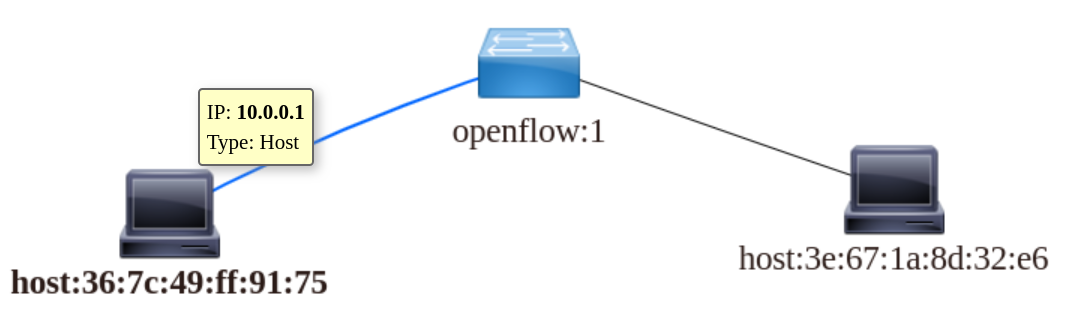
\includegraphics[scale=0.4]{figures/ch5/topo-simple}
	\caption{Single hop SDN topology emulated by mininet, and controlled by OpenDayLight Beryllium}
	\label{fig:topo-simple}
\end{figure}

All scripts used to create the scenarios, automate the tests, and cae the traffic, and the Octave scripts to perfom all thelable at the poject github repository\footnote{\href{https://github.com/AndersonPaschoalon/ProjetoMestrado/tree/master/Tests}{https://github.com/AndersonPaschoalon/ProjetoMestrado/tree/master/Tests}}. They are organized as a set of python packages to enable easy reproductionon Github\footnote{\textcolor{red}{github-link}}. To start rub and with all depencies installed, you should not take more than 10 minutes.

We will perform this testes using SIMITAR \textit{alpha} version, operation as a client on host \textit{h1}, and as a server on all other hosts. As traffic generator engine, we will use Iperf, D-ITG, and Libtins C++ API. 

\section{Simitar using Iperf and with skype-pcap}

\subsection{Single hop SDN topology}

We perform 


\begin{figure}[!ht]
	\centering
	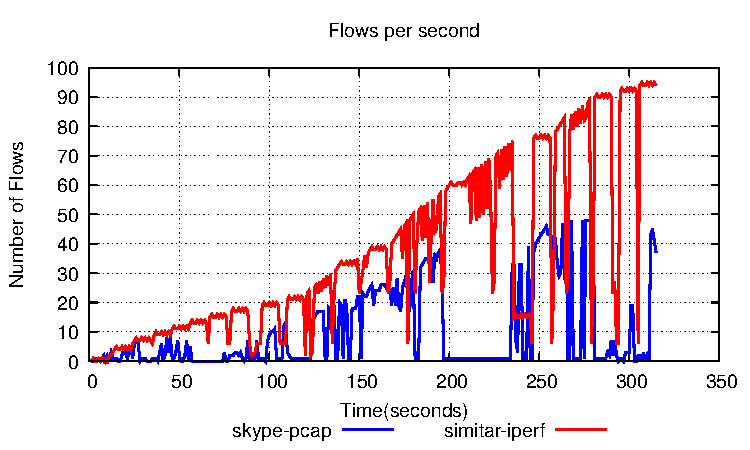
\includegraphics[scale=0.75]{figures/ch5/iperfFlowsPs.pdf}
	\caption{the caption}
	\label{fig:iperfFlowsPs}
\end{figure}

\begin{figure}[!ht]
	\centering
	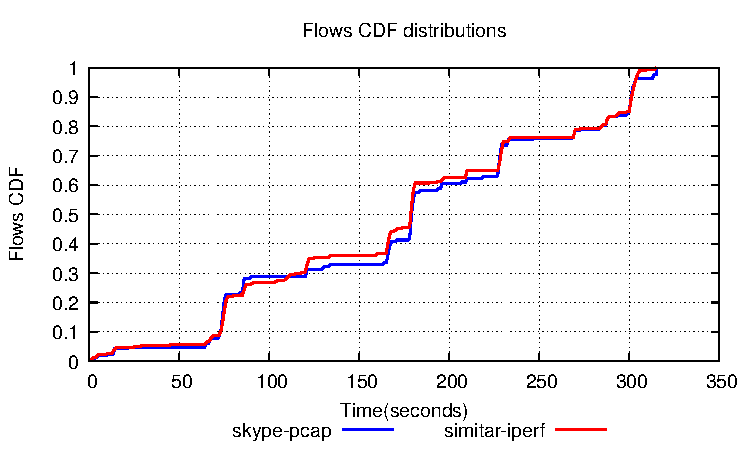
\includegraphics[scale=0.75]{figures/ch5/iperfFlowCdf.pdf}
	\caption{the caption}
	\label{fig:iperfFlowCdf}
\end{figure}

\begin{figure}[!ht]
	\centering
	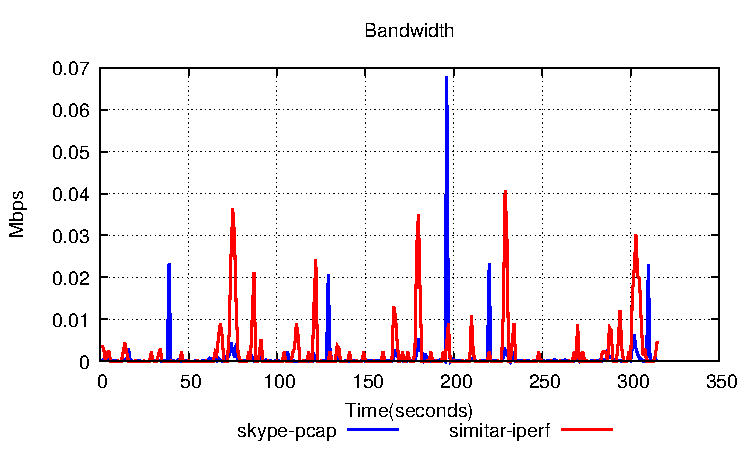
\includegraphics[scale=0.75]{figures/ch5/iperfBandwidth.pdf}
	\caption{the caption}
	\label{fig:iperfBandwidth}
\end{figure}

\begin{figure}[!ht]
	\centering
	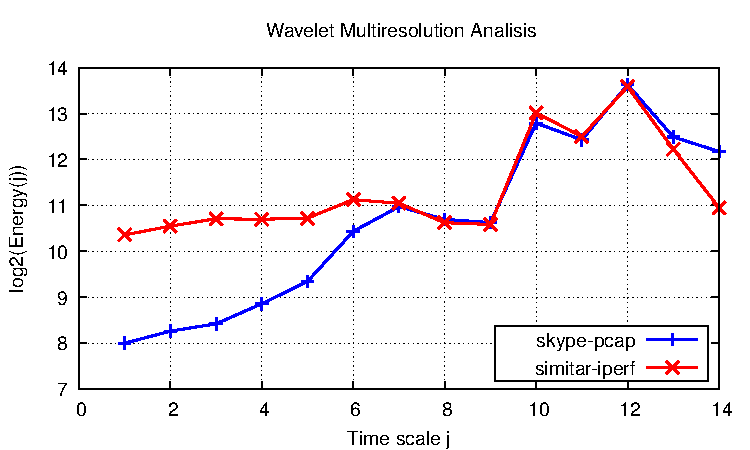
\includegraphics[scale=0.75]{figures/ch5/iperfWaveletMREA.pdf}
	\caption{the caption}
	\label{fig:iperfWaveletMREA}
\end{figure}

\subsection{Tree SDN topology}


\section{Simitar using D-ITG with skype-pcap}

\section{Simitar using Libtins with skype-pcap}


\section{Simitar lanDiurnal-pcap/bigFlows-pcap}


\subsection{Iperf as packetgen tool}


\subsection{Libtins as packetgen tool}



To evaluate the Scalling profile of the traccic generator, we are usig the same validation used for Swing\cite{swing-paper}: multiresolution energy analysis.
